\documentclass{beamer}
\usetheme{AnnArbor}
\usepackage{graphicx}
% Figures live one level up in ../figures relative to this .tex file
% Search both ../ (so includegraphics{figures/...} works) and ../figures/ (so includegraphics{...} works)
\graphicspath{{../}{../figures/}}
\usepackage{amsmath}
\usepackage{amssymb}
\usepackage  \begin{itemize}
    \item As $h$ decreases: $1.0 \to 0.5 \to 0.1 \to 0.01 \to 0$
    \item Secant slopes converge: $6.0 \to 5.0 \to 4.1 \to 4.01 \to 4$
    \item The limiting slope gives the exact tangent slope
  \end{itemize}
\end{frame}

\end{document}
\usepackage{tikz}
\usepackage[]{xcolor}
\usepackage[most]{tcolorbox}
\usepackage{pgfplots}
\pgfplotsset{compat=1.18}
\usepackage{blkarray}
\setbeamercolor{mycolorbox}{%
  bg=yellow!20,   % background color (20% yellow)
  fg=black      % foreground (text) color
}
\usefonttheme[onlymath]{serif}

\newtcolorbox{solutionblock}{
  colback=yellow!5,        % Background color: light yellow
  colframe=orange!80!black, % Frame color: dark orange
  title=Solution,
  fonttitle=\bfseries
}

\title{Introduction to Calculus}
\author{Nithin}
\institute{}
\date{\today}
\begin{document}
\begin{frame}
  \titlepage
\end{frame}
\begin{frame}
  \tableofcontents
\end{frame}


\begin{frame}{Chapter Overview}
\begin{itemize}
    \item<1-> \textbf{Historical Context:} Mathematicians of the 17th century were keenly interested in studying motion
    \begin{itemize}
        \item Objects on or near Earth
        \item Motion of planets and stars
    \end{itemize}
    
    \item<2-> \textbf{Key Insights:} Motion study involved both speed and direction
    \begin{itemize}
        \item Direction at any instant: along the tangent line to the path
        \item Need for precise mathematical tools
    \end{itemize}
    
    \item<3-> \textbf{The Limit Concept:} Fundamental to finding
    \begin{itemize}
        \item Velocity of moving objects
        \item Tangent lines to curves
    \end{itemize}
    
    \item<4-> \textbf{Function Behavior:} Limits help us distinguish between
    \begin{itemize}
        \item Continuous variation (small changes in $x$ → small changes in $f(x)$)
        \item Discontinuous behavior (jumps, erratic variation)
        \item Unbounded growth or decay
    \end{itemize}
    
    \item<5-> \textbf{Our Approach:} Develop limits intuitively, then formally
\end{itemize}
\end{frame}
\section{Slopes and Average Rate of Change}

% Slide: Motivation and Overview
\begin{frame}{Motivation: Why Study Change?}
  \begin{itemize}
    \item Calculus explores how quantities change : how change in one quantity is related to a change in anotherand provides tools for modeling these changes.
    \item Functions link inputs ($x$) to outputs ($y=f(x)$); we investigate how $y$ varies as $x$ moves over an interval.
    \item Real-world example: Predicting economic indicators, modeling speeds, and more.
  \end{itemize}
\end{frame}

% Slide: Defining Average Rate of Change
\begin{frame}{Average Rate of Change and Secant Lines}
  \begin{block}{Definition}
    For a function $f(x)$ on interval $[x_{1},x_{2}]$, the \emph{average rate of change} over that interval is
    \[ 
      = \frac{\Delta y}{\Delta x} = \frac{f(x_{2})-f(x_{1})}{x_{2}-x_{1}} = \frac{f(x_{1}+h) - f(x_{1})}{h}, h \neq 0
    \]
    which geometrically represents the slope of the secant line between $(x_{1},f(x_{1}))$ and $(x_{2},f(x_{2}))$.
  \end{block}
  \begin{itemize}
    \item Rise: $f(x_{2})-f(x_{1})$
    \item Run: $x_{2}-x_{1}$
    \item The secant line smooths out fluctuations; its slope reports the net change per unit input over the interval.
    \item Approximating the curve over the interval with a straight line. 
  \end{itemize}
\end{frame}

% Slide: Graphical Illustration
\begin{frame}{Graphical Illustration}
  \begin{columns}
    \column{0.6\textwidth}
      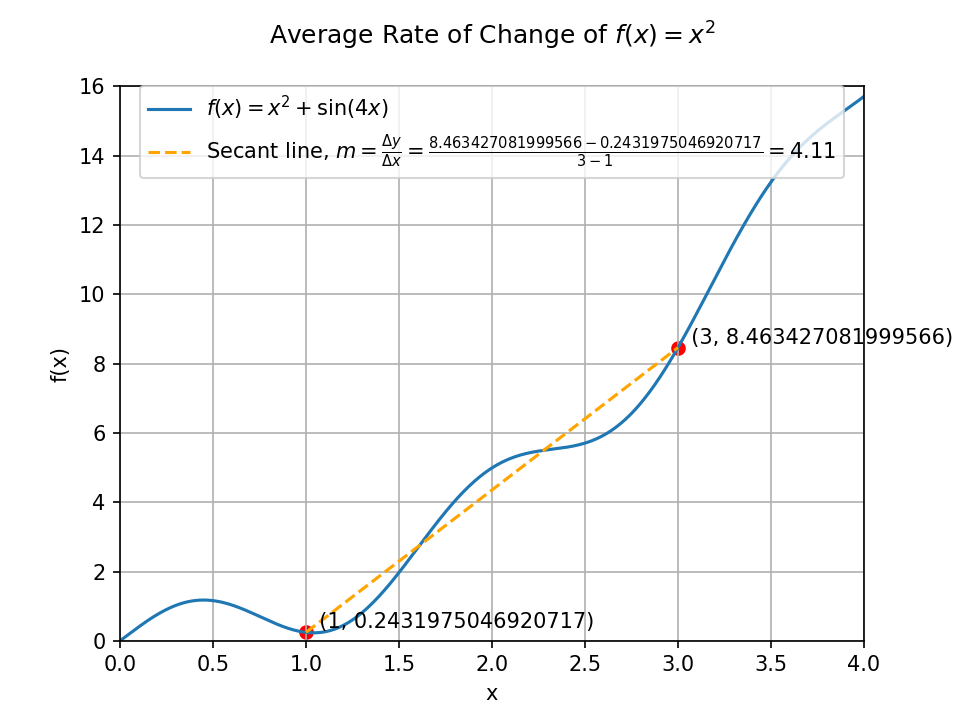
\includegraphics[width=\textwidth]{figures/avg_rate_of_change.png}
    \column{0.4\textwidth}
      \begin{itemize}
        \item Focus on interval $[1,3]$ on the curve $y=f(x)$.
        \item Secant line (in orange) joins $(1,f(1))$ and $(3,f(3))$.
        \item Its slope measures the average change in $y$ per unit change in $x$.
      \end{itemize}
  \end{columns}
\end{frame}

% Slide: Problem – Trivandrum to Chennai Average Speed
\begin{frame}{Example: Trivandrum to Chennai Journey}
  \begin{columns}
    \column{0.5\textwidth}
      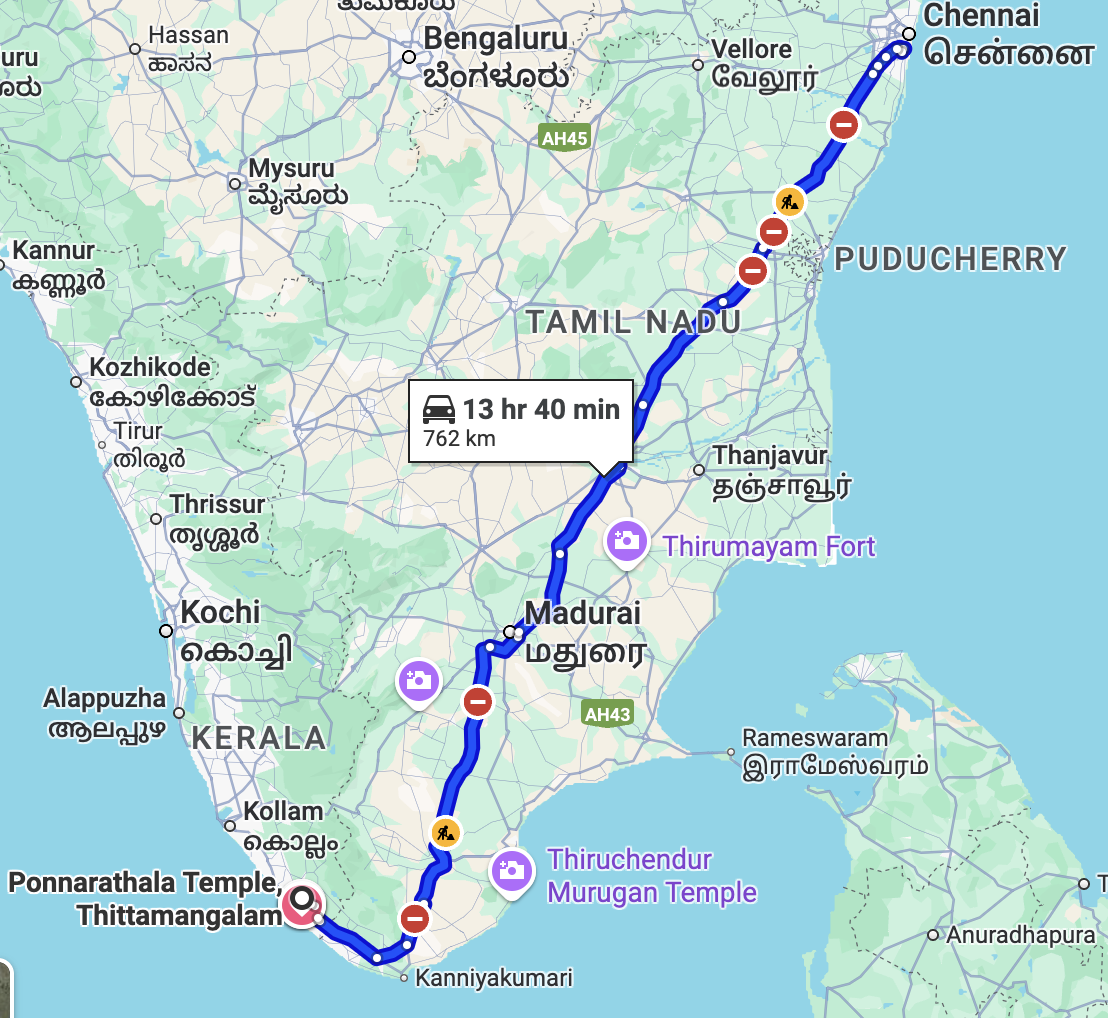
\includegraphics[width=\textwidth]{figures/trivandrum_chennai_map.png}
    \column{0.5\textwidth}
      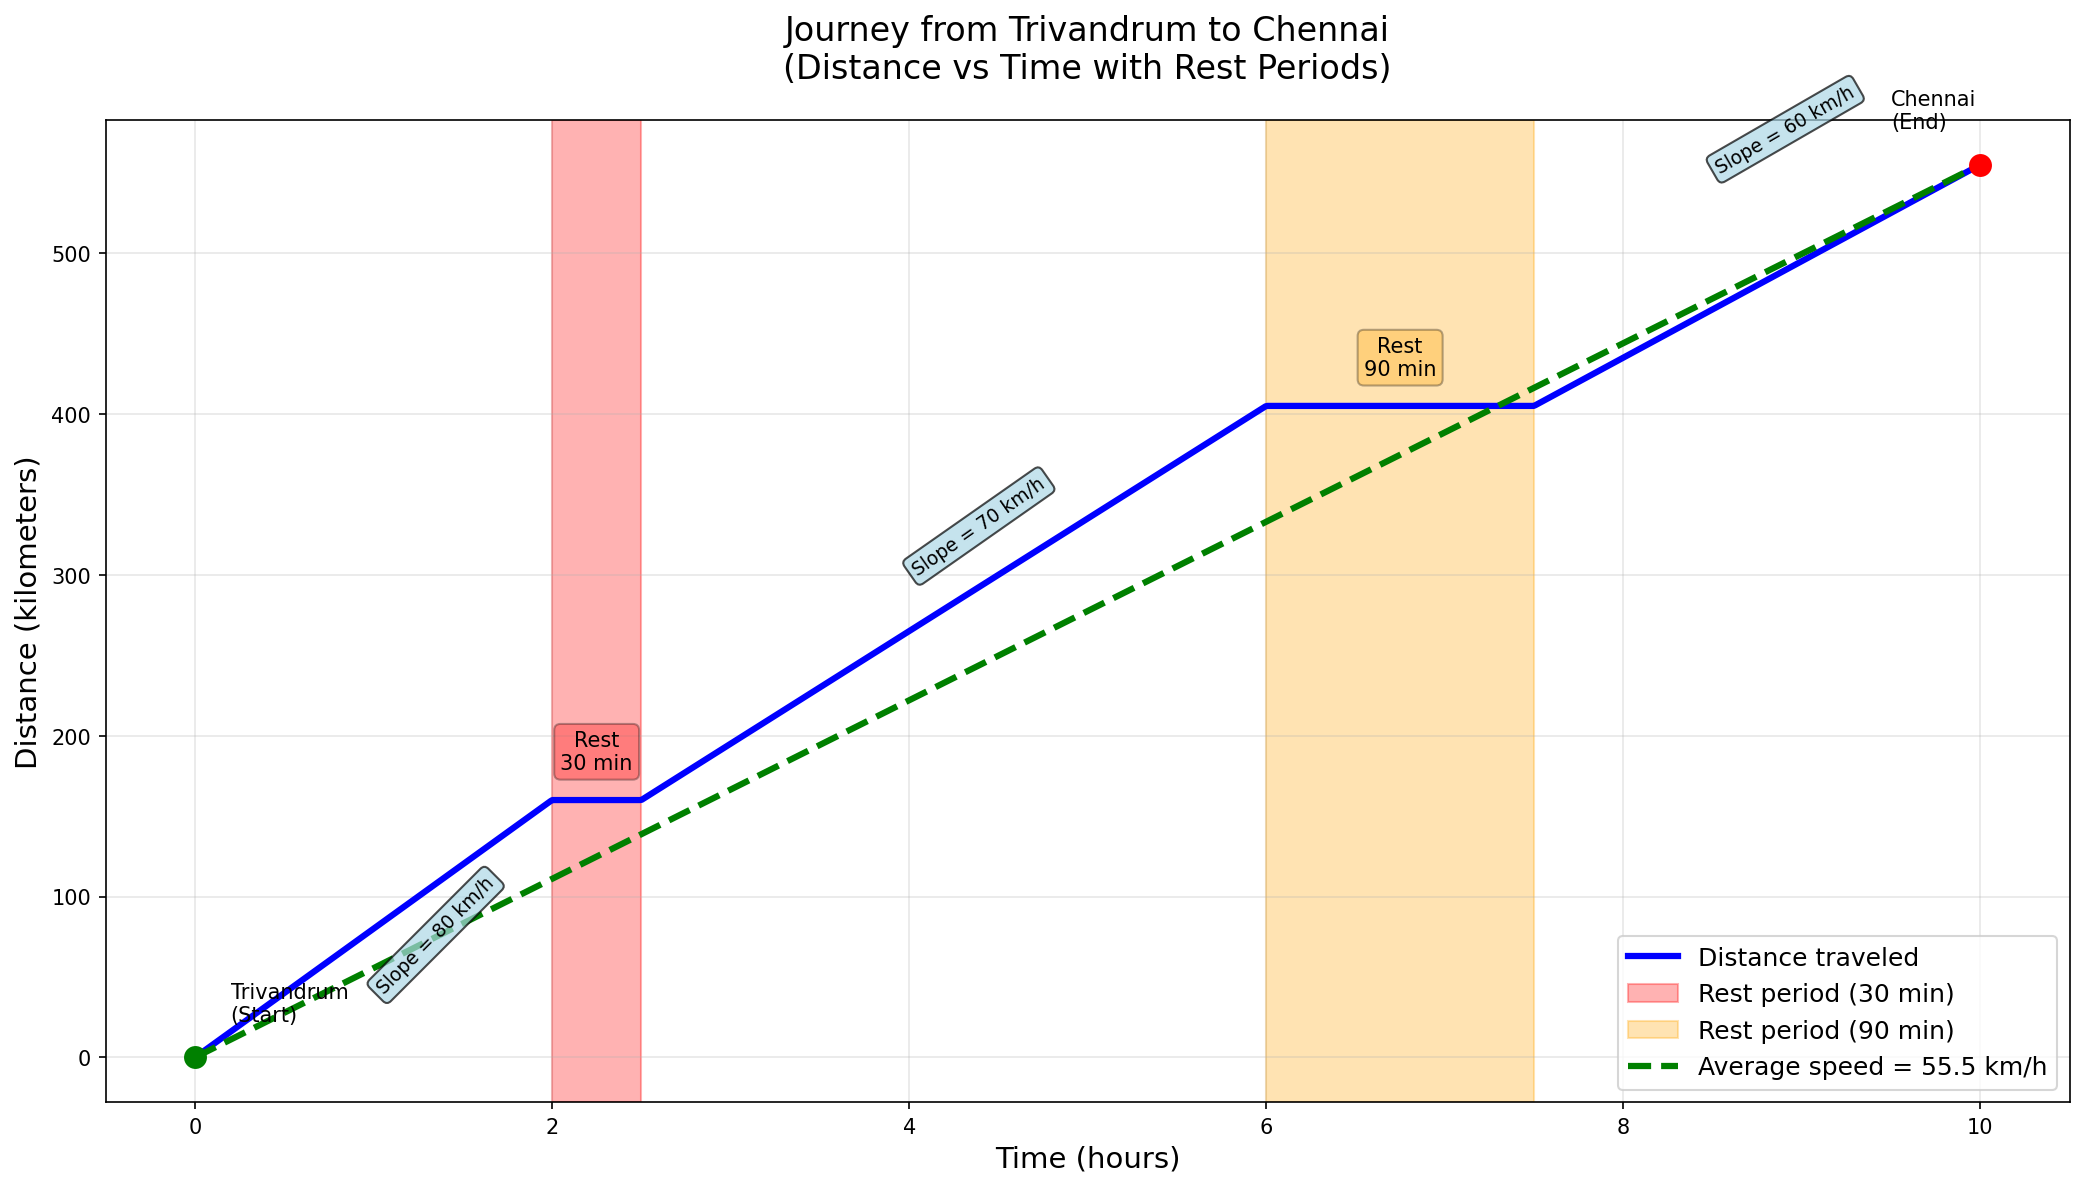
\includegraphics[width=\textwidth]{figures/trivandrum_chennai_journey.png}
  \end{columns}
  \vspace{1ex}

\end{frame}

\begin{frame}
  \begin{itemize}
    \item Total distance: 762 km
    \item Total time (including stops): 15 hours
    \item Average speed: $\dfrac{762}{15}\approx50.8$ km/h
  \end{itemize}
  \begin{solutionblock}
    Average speed $=\dfrac{\text{distance}}{\text{time}}=\dfrac{762}{15}\approx50.8\text{ km/h}$.  
  This illustrates how the secant slope over an interval gives overall performance even with rest periods.
  \end{solutionblock}
\end{frame}

% Slide: Sensitivity to Rounding
\begin{frame}{Rounding and Accuracy}
  \begin{columns}
    \column{0.58\textwidth}
      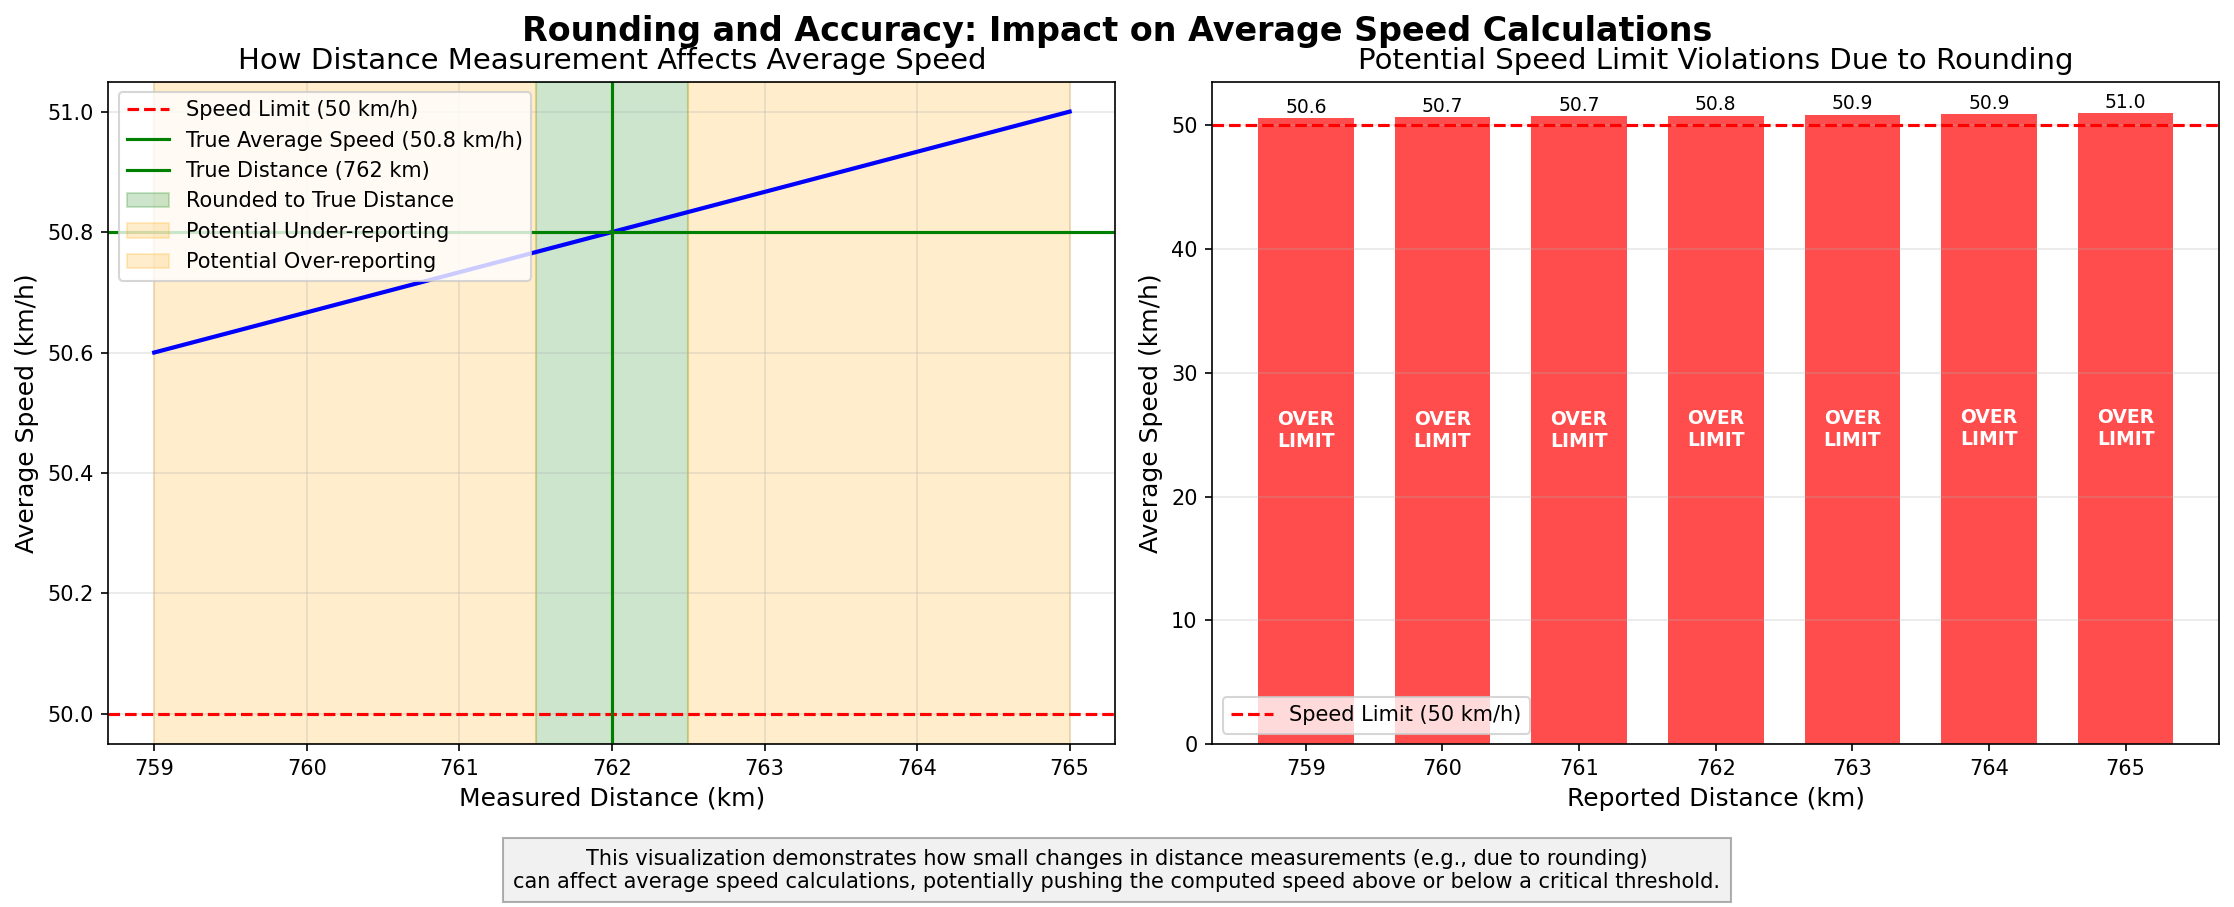
\includegraphics[width=\textwidth]{figures/rounding_accuracy_demo.png}
    \column{0.42\textwidth}
      \begin{itemize}
        \item Distance measurements rounded to nearest kilometer introduce potential error
        \item For our journey: $\dfrac{762\text{ km}}{15\text{ h}} \approx 50.8$ km/h
        \item A mere 3 km error in measurement can push calculated speed above/below the 50 km/h limit
        \item Data precision is important.
      \end{itemize}
  \end{columns}
\end{frame}

% Slide: Toward Instantaneous Rate of Change
\begin{frame}{Instantaneous Rate of Change}
  \begin{itemize}
    \item Instantaneous speed corresponds to slope of tangent line at a point.
    \item As secant interval shrinks ($b\to a$), average rate approaches derivative $f'(x)$.
    \item Next: Formalize tangent lines and derivatives.
  \end{itemize}
\end{frame}

\begin{frame}
\frametitle{Why Instantaneous Rate of Change?}
\begin{itemize}
  \item Average rate of change provides overall performance but lacks detail.
  \item Instantaneous rate of change captures behavior at a specific moment while average rate is over an interval
  \item Essential for understanding dynamic systems (e.g., velocity, acceleration).
  \item Instantaneous rate of change = calculate average rathe of change over smaller and smaller intervals.
\end{itemize}
\end{frame}
\begin{frame}{Secants to Tangents}
  \centering
  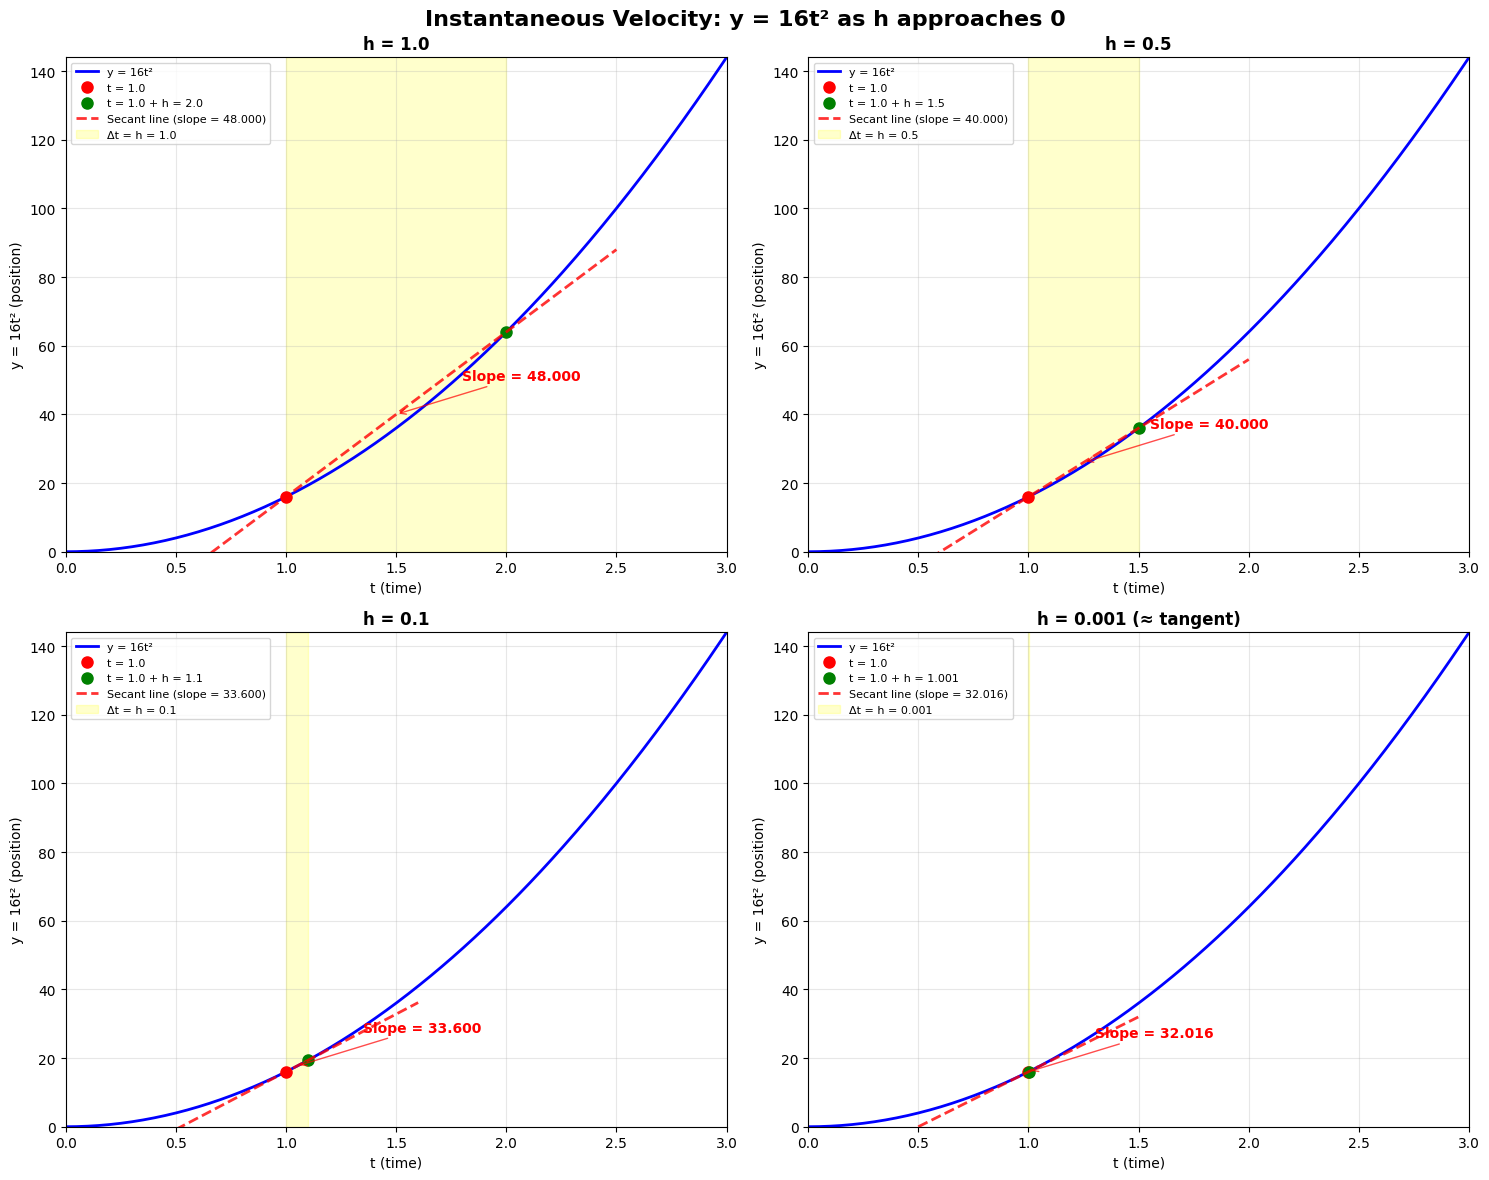
\includegraphics[width=0.8\textwidth]{figures/instantaneous_rate_change.png}
\end{frame}

\begin{frame}
  \frametitle{The Mean Value Theorem}
  \begin{figure}
    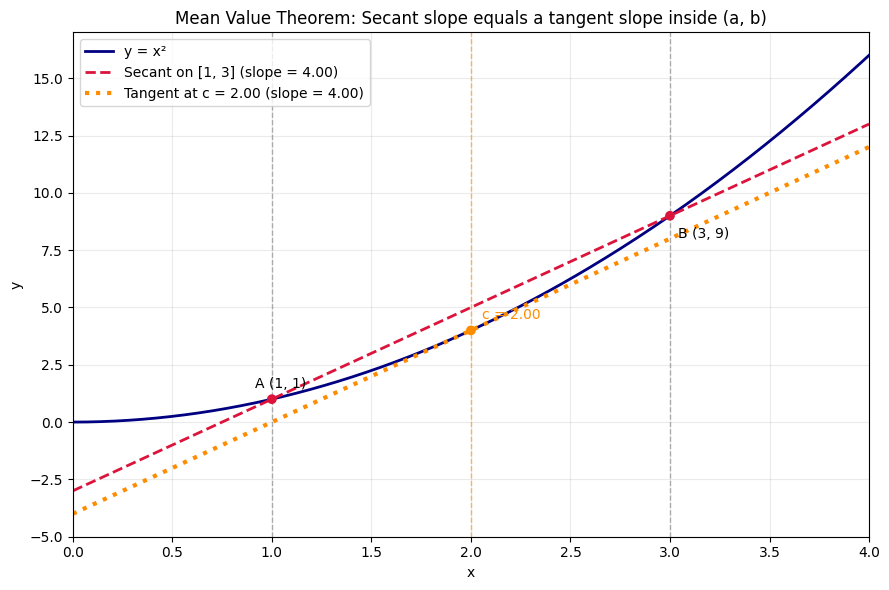
\includegraphics[width=0.75\textwidth]{figures/mean_value.png}
    \caption{Mean Value Theorem: There exists a point $c$ where the tangent equals the secant.}
  \end{figure}
\end{frame}
% Slide: Mean Value Theorem (informal, no derivatives)
\begin{frame}{The Mean Value Theorem (informal, no derivatives)}
  \begin{block}{Statement}
  For a smooth curve $y=f(x)$ on an interval $[a,b]$, the \emph{average rate of change}
  \[ \dfrac{f(b)-f(a)}{b-a} \]
  is realized as the slope of a \emph{tangent line} at some point $x=c$ with $a<c<b$.
  In other words, the secant line joining $(a,f(a))$ and $(b,f(b))$ has the same slope as
  the tangent line to the curve at some point inside the interval.
  \end{block}
  \vspace{0.5em}
\end{frame}
\section{Displacement, Velocity, and Acceleration}
\begin{frame}{Displacement}
  \begin{block}{Definition}
    The displacement $x(t)$ at time $t$ measures position on the real line relative to an origin $0$, so positive values indicate one direction and negative values the opposite.
  \end{block}
  \begin{itemize}
    \item Independent variable: time $t$ (typically seconds).
    \item Dependent variable: displacement $x$.
    \item Choice of origin and direction provides a signed measure of position.
  \end{itemize}
\end{frame}

\begin{frame}{Velocity}
  \begin{block}{Definition}
    The velocity $v(t)$ is the instantaneous rate of change of displacement $x(t)$.
  \end{block}
  \begin{itemize}
    \item $v(t)>0$ (motion in the positive direction), $v(t)<0$ (negative direction), or $v(t)=0$.
    \item Speed is the magnitude of velocity: $\text{speed}=\lvert v(t)\rvert$.
    \item A speedometer displays instantaneous speed.
  \end{itemize}
\end{frame}

\begin{frame}{Acceleration}
  \begin{block}{Definition}
    The acceleration $a(t)$ is the instantaneous rate of change of velocity $v(t)$.
  \end{block}
  \begin{itemize}
    \item $a(t)$ may be positive, negative, or zero.
    \item The term “deceleration” is often used when $a(t)$ is negative and quoted as a positive number by convention.
  \end{itemize}
\end{frame}

\begin{frame}{Example: Cannonball Projectile}
  \begin{figure}
    \centering
    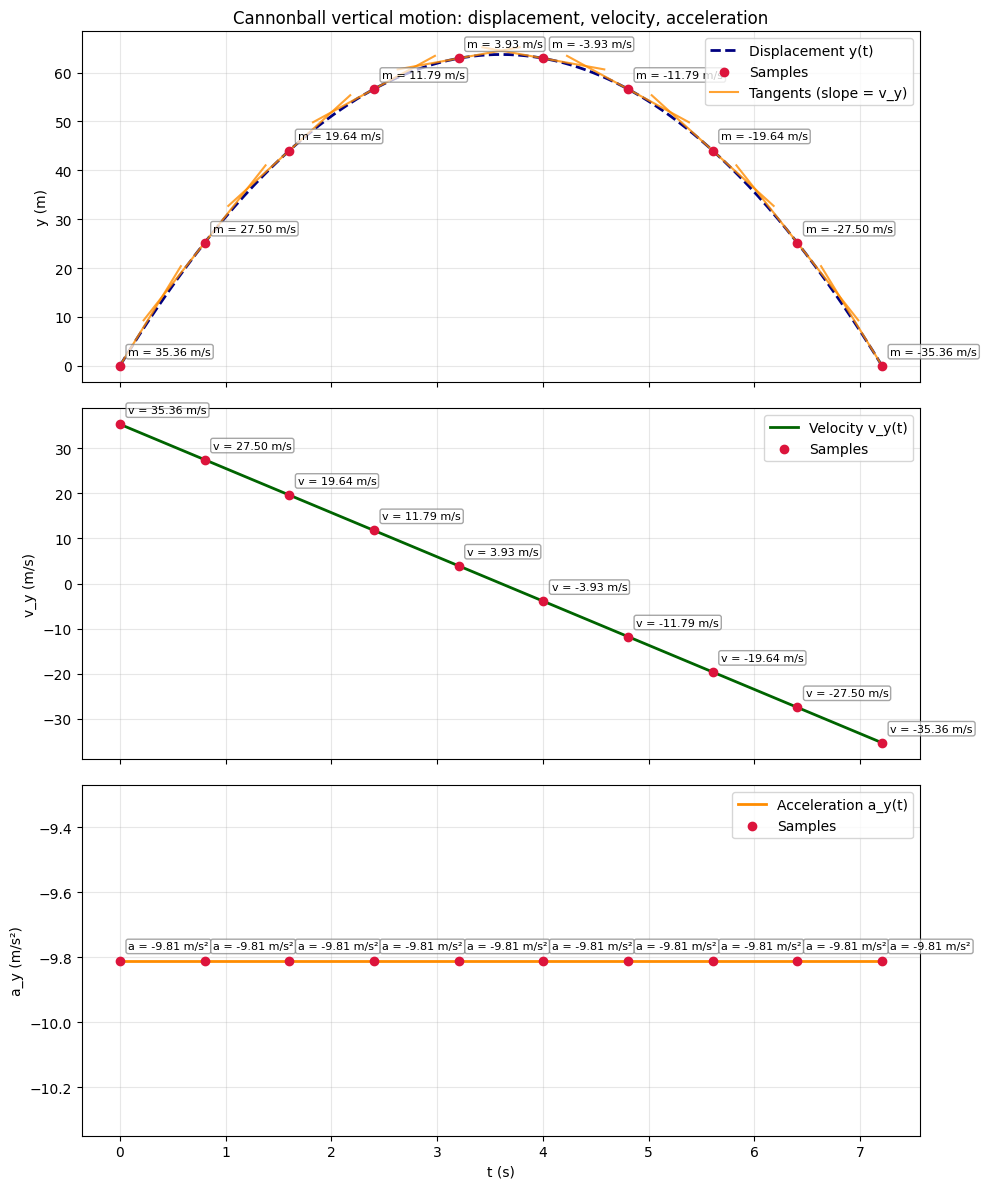
\includegraphics[width=0.5\textwidth]{figures/cannonball.png}
  \end{figure}
\end{frame}

\section{First Principle: Finding the Derivative}

\begin{frame}{First Principle Method}
  \begin{block}{Problem}
    Find the slope of the parabola $y = x^2$ at the point $P(2, 4)$ using the first principle (limiting of secant lines).
  \end{block}
  
  \begin{block}{First Principle Formula}
    The derivative (slope of tangent) at $x = a$ is:
    \[ f'(a) = \lim_{h \to 0} \frac{f(a+h) - f(a)}{h} \]
  \end{block}
  
  \begin{itemize}
    \item<2-> For $f(x) = x^2$ and $a = 2$:
    \[ f'(2) = \lim_{h \to 0} \frac{f(2+h) - f(2)}{h} = \lim_{h \to 0} \frac{(2+h)^2 - 4}{h} \]
    
    \item<3-> Expanding: $(2+h)^2 = 4 + 4h + h^2$
    \[ f'(2) = \lim_{h \to 0} \frac{4 + 4h + h^2 - 4}{h} = \lim_{h \to 0} \frac{4h + h^2}{h} \]
    
    \item<4-> Factoring and simplifying:
    \[ f'(2) = \lim_{h \to 0} \frac{h(4 + h)}{h} = \lim_{h \to 0} (4 + h) = 4 \]
  \end{itemize}
\end{frame}

\begin{frame}{Numerical Convergence: Code Implementation}
  \begin{block}{Python Code Demonstration}
    For $f(x) = x^2$ at point $(2, 4)$:
    \begin{center}
    \texttt{slope = (f(2 + h) - f(2)) / h}
    \end{center}
  \end{block}
  
  \begin{columns}
    \column{0.5\textwidth}
    \begin{table}
    \centering
    \begin{tabular}{|c|c|}
    \hline
    $h$ & Slope \\
    \hline
    $1.000$ & $6.000000$ \\
    $0.500$ & $5.000000$ \\
    $0.100$ & $4.100000$ \\
    $0.010$ & $4.010000$ \\
    $0.001$ & $4.001000$ \\
    $0.0001$ & $4.000100$ \\
    \hline
    \end{tabular}
    \end{table}
    
    \column{0.5\textwidth}
    \begin{itemize}
      \item<2-> As $h \to 0$, slope $\to 4$
      \item<3-> \textbf{Code verification:}
      \begin{align}
        \text{slope} &= \frac{(2+h)^2 - 4}{h} \\
        &= \frac{4 + 4h + h^2 - 4}{h} \\
        &= \frac{4h + h^2}{h} \\
        &= 4 + h
      \end{align}
      \item<4-> When $h = 0.001$: slope $= 4.001$
      \item<5-> Limit: $\lim_{h \to 0}(4 + h) = 4$
    \end{itemize}
  \end{columns}
\end{frame}

\begin{frame}{Solution: Tangent Line at P(2, 4)}
  \begin{solutionblock}
    \textbf{Step 1:} Using first principle, we found $f'(2) = 4$
    
    \textbf{Step 2:} The slope of the tangent line at $P(2, 4)$ is $m = 4$
    
    \textbf{Step 3:} Using point-slope form: $y - y_1 = m(x - x_1)$
    \[ y - 4 = 4(x - 2) \]
    
    \textbf{Step 4:} Simplifying:
    \[ y = 4x - 8 + 4 = 4x - 4 \]
    
    \textbf{Final Answer:}
    \begin{itemize}
      \item Slope at $P(2, 4)$: $m = 4$
      \item Tangent line equation: $y = 4x - 4$
    \end{itemize}
  \end{solutionblock}
\end{frame}

\begin{frame}{Visualization: Secant Lines Approaching Tangent}
  \begin{figure}
    \centering
    % This figure would be generated from the Python code and saved
    \includegraphics[width=0.9\textwidth]{figures/first_principle_demo.png}
    \caption{Secant lines with decreasing $h$ values approaching the tangent line at $P(2, 4)$}
  \end{figure}
  
  \begin{itemize}
    \item As $h$ decreases: $1.0 \to 0.5 \to 0.1 \to 0.01 \to 0$
    \item Secant slopes converge: $6.0 \to 5.0 \to 4.1 \to 4.01 \to 4$
    \item The limiting slope gives the exact tangent slope
  \end{itemize>
\end{frame}

\end{document}